\section{Decision Trees}\label{s:decision-trees}

Decision trees are tree-like structures in which each internal node represents a ``test" on an attribute, each branch represents the outcome of the specific test, and each leaf node represents a class label (decision taken after computing all attributes).
More specifically, decision trees depict models of decisions and their possible results.
They are also a simple way to display an algorithm that only contains conditional control statements.
Starting from the root node and following the paths to leaves, each path represents classification rules.

For instance, the attribute ``Gender" would have two edges leaving it, one for ``Male" and
one for ``Female".
Each edge could point to a new attribute (for example ``Age Groups"), and so on.
The leaves of the tree contain the expected class value for transactions matching the path from the root to that leaf.
Given a decision tree, one can predict the class of a new transaction just by following the ``correct" path, which will result in a class label.
He/She can predict the class of a transaction by viewing only the non-class attributes (i.e. the ``constructed" decision tree).

For instance, two friends wish to decide if they will go to play tennis outside, depending the weather conditions.
They also remember the previous days that some weather conditions did not allow them to play.
Thus, they decide to create a decision tree to assist them.
First they define the class attribute to be ``Play Tennis", and three more attributes that will help them decide: ``Outlook" (``Sunny", ``Overcast", ``Rainy"), ``Windy" (``High", ``Low") and ``Humidity" (``High", ``Low").
Then they construct a decision tree like figure \ref{f:outlook} that corresponds to the data that the have collect from the past days.

\begin{figure}[t]
  \centering
  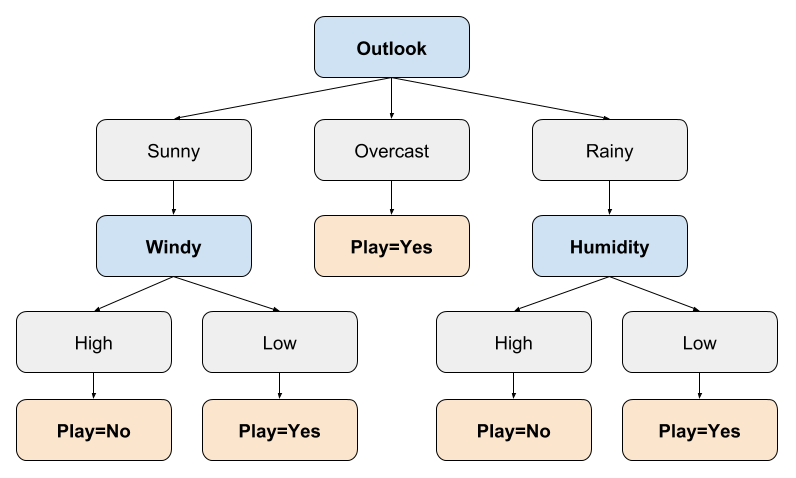
\includegraphics[width=0.8\linewidth]{figures/outlook.png}
  \caption{Play-Tennis decision tree example}\label{f:outlook}
\end{figure}

From figure \ref{f:outlook}, the two friends are able to extract a set of rules, listed in Code \ref{sc:outlook-rules}, that will help them decide if they should go play tennis given the weather conditions.

{
\begin{minted}[xleftmargin=21pt, framesep=3mm, frame=single, linenos, tabsize=2, breaklines, breaksymbolleft=, fontsize=\footnotesize]{bash}
IF (Outlook = Sunny) AND (Windy = Low) THEN Play=Yes

IF (Outlook = Sunny) AND (Windy = High) THEN Play=No

IF (Outlook = Overcast) THEN Play=Yes

IF (Outlook = Rainy) AND (Humidity = High) THEN Play=No

IF (Outlook = Rainy) AND (Humidity = Low) THEN Play=Yes
\end{minted}
\captionof{lstlisting}{Rules for decision tree from figure \ref{f:outlook}}
\label{sc:outlook-rules}
}

Of course, remembering the weather conditions of more days in the past and if they had played tennis those days -- having an extended dataset -- could probably result to more specific rules.
Decision tree rules, help covering all possible future decisions\hyp transactions and can be used to classify them.
There are many useful examples and it has become evident why this type of learning has become so popular.
The algorithms according to which those tress are generated vary and lead to possible different trees.

One famous algorithm for decision tree construction is ID3 (Iterative Dichotomiser 3).
ID3 is the precursor to the C4.5 algorithm, and is typically used in the machine learning and natural language processing domains.
Both algorithms build decision trees from a set of training data, using the concept of information entropy, however, C4.5 results in better classification utilizing a more efficient splitting criterion.




\subsection{Textbook ID3}\label{s:id3}

The ID3 algorithm was first introduced in \cite{quinlan1986induction} and assumes that each attribute is categorical, such as the aforementioned attribute ``Age Groups" which is separated in four disjoint categories; ``Infant", ``Adolescent", ``Child" and ``Adult".

ID3 algorithm constructs the classification tree top-down in a recursive fashion.
The idea is to find the \textit{best} attribute that classifies the transactions.
At start, the algorithm searches and chooses the best attribute for the root node, and consecutively the remaining transactions are partitioned by it.
On each partition, ID3 is then recursively called.

The \textit{best} attribute is defined as the attribute that has the smallest entropy -- or in other words, the best information gain.
Let $T$ be a set of transactions, $C$ the class attribute and $A$ some non-class attribute.
On each iteration, ID3 iterates through every unused attribute $A$ of the dataset and calculates the entropy $H_C(T)$ (equation \ref{eq:entropy} and algorithm \ref{a:id3-Entropy-simple}) for every subset $T$ that results from splitting the dataset on attribute $A$.

\import{./}{algorithms/entropy_textbook.tex}

\begin{equation}\label{eq:entropy}
  H_C(T) = \sum_{i=1}^{l} - \frac{\mid T(c_i) \mid}{\mid T \mid} log{\frac{\mid T(c_i) \mid}{\mid T \mid}}
\end{equation}

The idea is to identify the class of a transaction $t$, given that the value of $A$ has been obtained.
Let $A$ obtain values $a_1, \dots, a_m$ and let $T(a_j)$ be the transactions obtaining value $a_j$ for $A$.
Then, the conditional information of $T$ given $A$, is given from equation \ref{eq:TgivenA}.

\import{./}{algorithms/gain_textbook.tex}

\import{./}{algorithms/best_textbook.tex}

\begin{equation}\label{eq:TgivenA}
  H_C(T \mid A) = \sum_{j=1}^{m} - \frac{\mid T(a_j) \mid}{\mid T \mid} H_C(T(a_j))
\end{equation}

\begin{equation}\label{eq:gain}
  Gain(A) = H_C(T) - H_C(T \mid A)
\end{equation}


Finally, the set $T$ is then split by the selected attribute $A$ (best-attribute algorithm \ref{a:id3-best-simple}) that has the maximum gain (equation \ref{eq:gain} and algorithm \ref{a:id3-gain-simple}) -- or equivalently minimum $H_C(T \mid A)$ -- to produce subsets of the data.
The algorithm continues to recurse on each subset, considering only attributes never selected before.


\import{./}{algorithms/allsame_textbook.tex}

\import{./}{algorithms/id3_textbook.tex}



\subsection{Privacy Preserving ID3}\label{s:pp-id3}

\fixme{many things from \href{http://www.pinkas.net/PAPERS/id3-final.pdf}{http://www.pinkas.net/PAPERS/id3-final.pdf}}

In privacy-preserving algorithms, all intermediate values should remain hidden.
In many cases, intermediate values may reveal some patterns, and in general sensitive information about the inputs.

However, in the case of ID3, some of these intermediate values are part of the output and eventually will be revealed.
For instance, the attributes chosen in each node of the tree will be revealed in the final results.
Thus, there is no reason to trying to protect them during the protocol execution.
In the privacy-preserving ID3, as in all algorithms in this thesis, we explicitly define which values are private (and thus encrypted), and which are public.

Although the names of the selected attributes will be revealed (those nodes have the highest information gain), nothing is learned about the actual $H_C(T \mid A)$ values themselves.
Therefore, the problem is reduced to privately find the attribute with the highest information gain.

Despite the fact that the selected attributes will be revealed, we cannot regard their values as public data.
All computations are carried out on encrypted data -- using the homomorphic properties of secret sharing, and when a decision is made ....
\fixme{explain more here}



As we have mentioned, our aim is to privately find the attribute $A$ for which $H_C(T \mid A)$ is minimum....
\fixme{explain PP-Best, PP-Gain and PP-Entropy!}


\import{./}{algorithms/id3_pp.tex}




\subsection{Textbook C4.5}\label{s:c45}

\subsection{Privacy Preserving C4.5}\label{s:pp-c45}


